%===============================================================================
%===============================================================================
%
\subsection{Example-0101}
%
%===============================================================================
%
\subsubsection{Model}
%
We solve the following equation,
%
\begin{align}
    \nabla \cdot \boldsymbol{\sigma} (\boldsymbol{u}, t) = \boldsymbol{0} (\boldsymbol{u}, t) & &&\Omega \in [0, 160] \times [0, 120], t \in [0, 5],
\end{align}
%
with time step size $\Delta_t = 1$ and boundary conditions
%
\begin{align}
    \ldots & && \ldots, \\
    \ldots & && \ldots.
\end{align}
%
2D: specify thickness, Young's modulus and Poisson's ratio.
%
%===============================================================================
%
\subsubsection{Results}
%
\begin{figure}[h!]
    \centering 
    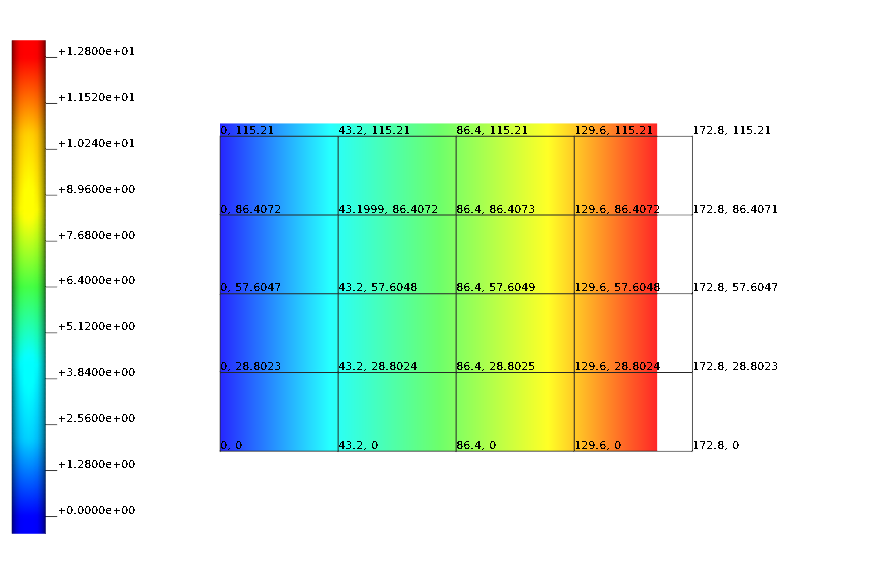
\includegraphics[width=\columnwidth]{examples/example-0101/figures/example.png} 
    \caption{Results.}
    \label{example-0101-fig}
\end{figure}
%
%===============================================================================
%===============================================================================
